\chapter{Materiali e metodi}
\label{chap:materiali_metodi}

\section{Dataset RHPE}
\label{sec:dataset}

Il dataset RHPE (Radiological Hand Pose Estimation) è composto da radiografie
della mano di pazienti pediatrici, suddivise nei tre split standard di
training, validation e test (Sez.~\ref{sec:classificazione}). Le
annotazioni sono fornite in due formati:

\begin{itemize}
    \item \textbf{JSON (formato COCO):} bounding box della mano e 17
    keypoint anatomici codificati come triplette $(x, y, v)$, dove $v$
    rappresenta il flag di visibilità;
    \item \textbf{CSV:} età ossea (\emph{bone age}), età cronologica e
    genere per ogni paziente.
\end{itemize}

Il test set non include l'età ossea, poiché è il valore che il sistema deve
predire.

Le radiografie della mano acquisite in ambito clinico mostrano
tipicamente entrambe le mani sulla stessa immagine, per permettere un
confronto diretto tra i due lati, ed è così anche per le immagini
fornite da RHPE: ogni file mostra entrambe le mani, ma le annotazioni
(bounding box e keypoint) riguardano esclusivamente la mano sinistra
(non dominante), presente per convenzione nella metà sinistra
dell'immagine. Questo aspetto è rilevante per il lavoro di estensione
alla mano destra descritto in Sez.~\ref{sec:esplorazione_dx_metodo}.

\subsection{Analisi esplorativa}
\label{sec:eda}

\begin{table}[H]
\centering
\caption{Distribuzione del dataset RHPE per split.}
\label{tab:dataset_split}
\begin{tabular}{lccc}
\toprule
Split & Immagini & Maschi & Femmine \\
\midrule
Train & 5491 & 2372 (43.2\%) & 3119 (56.8\%) \\
Val   & 713  & 306 (42.9\%)  & 407 (57.1\%)  \\
Test  & 79   & 38 (48.1\%)   & 41 (51.9\%)   \\
\bottomrule
\end{tabular}
\end{table}

\begin{figure}[H]
\centering
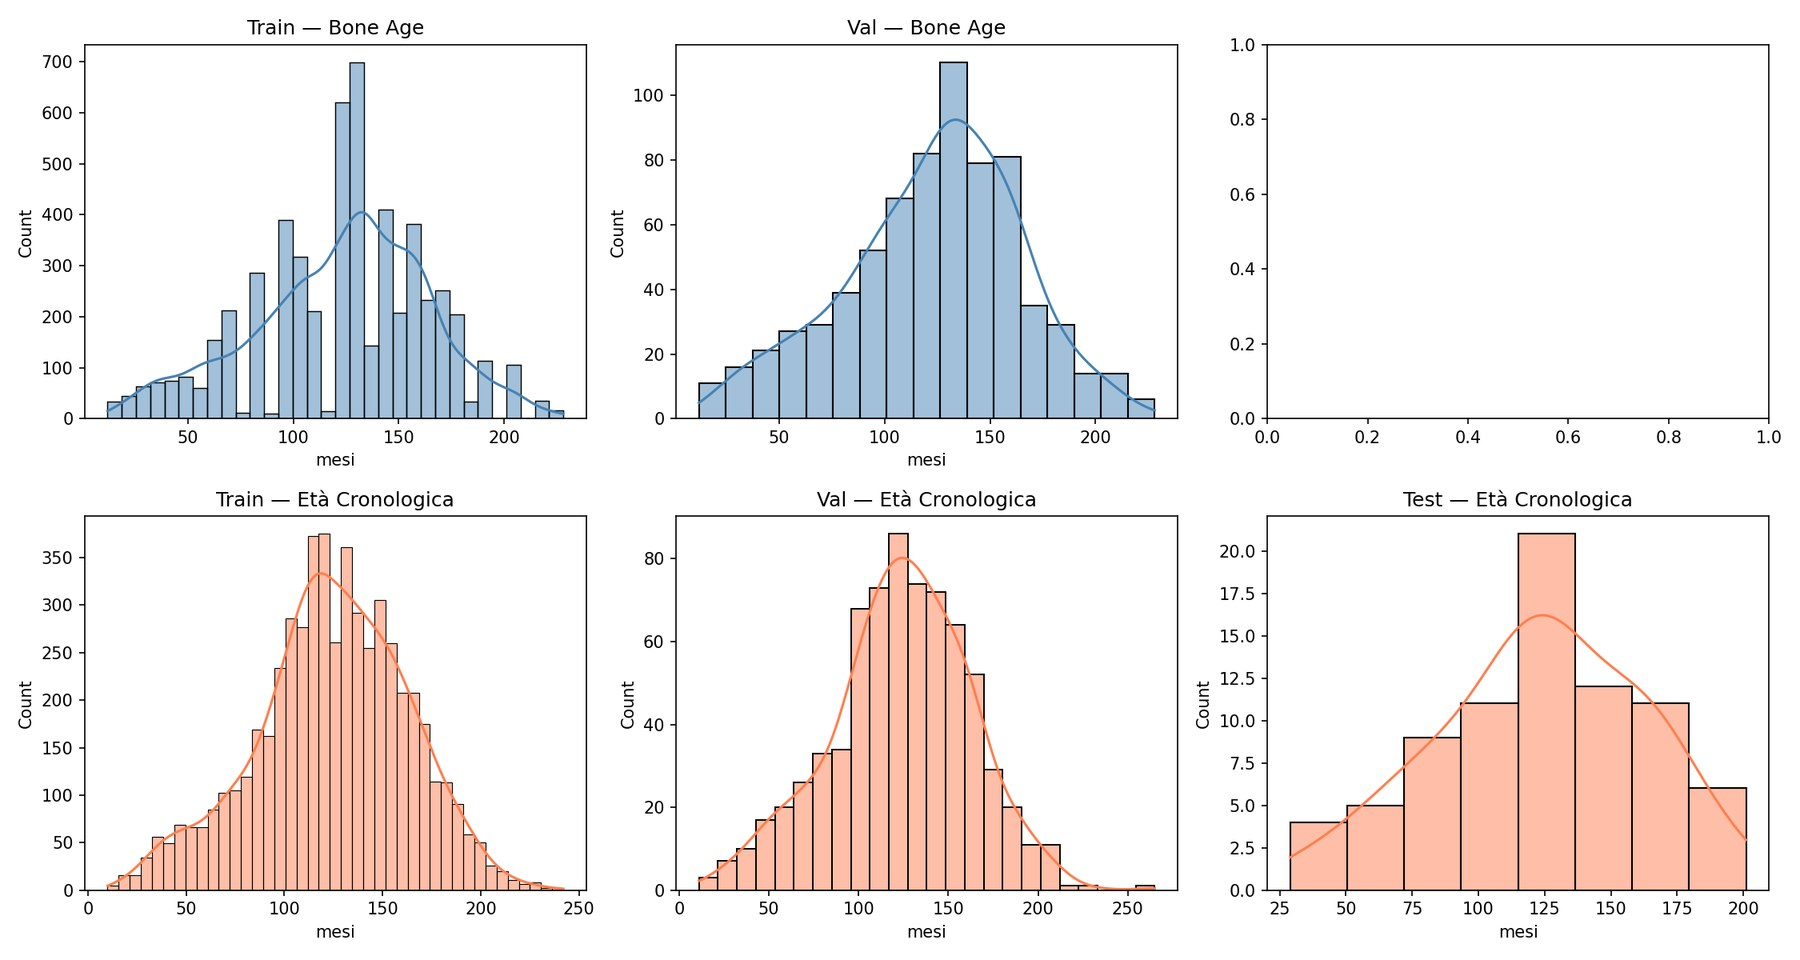
\includegraphics[width=0.95\textwidth]{figure/distribuzione_eta.jpg}
\caption{Distribuzione di bone age ed età cronologica sui tre split del dataset RHPE.}
\label{fig:distribuzione_eta}
\end{figure}

\section{Hand Detection}
\label{sec:hand_detection}

Il primo stadio della pipeline consiste nel localizzare automaticamente la
mano nell'immagine tramite bounding box. Seguendo il paper BoNet, il
modello scelto è Faster R-CNN con backbone ResNet-50 FPN, pre-addestrato su
ImageNet (Sez.~\ref{sec:architetture}). L'architettura viene adattata al task tramite fine-tuning:
l'ultimo layer (\texttt{box\_predictor}), originariamente configurato per
91 classi (dataset COCO), viene sostituito con uno nuovo per 2 classi
(background e mano).

\subsection{Campionamento stratificato}

Su indicazione del supervisore, i sottoinsiemi utilizzati per la hand 
detection sono composti da 250 immagini di training e 50 di validation.
Anziché utilizzare le prime $N$ immagini del training set, per la
costruzione dei sottoinsiemi di training e validation è stato adottato
un campionamento stratificato per fascia d'età, con fasce di ampiezza 24
mesi. Questa scelta garantisce che il sottoinsieme utilizzato per
l'addestramento sia rappresentativo dell'intera distribuzione delle età
del dataset, evitando che alcune fasce risultino sovra- o
sotto-rappresentate rispetto ad altre. 

\subsection{Collegamento tra annotazioni CSV e JSON}

Un aspetto non banale nella costruzione del dataset riguarda il
collegamento tra le informazioni provenienti dai due formati di
annotazione disponibili. Il file CSV identifica ciascun paziente tramite
un ID progressivo (1, 2, 3, \dots), mentre il file JSON in formato COCO
assegna a ciascuna immagine un ID interno arbitrario (ad esempio 3722) e
un nome file (ad esempio \texttt{00001.png}). L'unico elemento in comune
tra le due annotazioni è il numero progressivo codificato nel nome del
file, che corrisponde all'ID utilizzato nel CSV. Il dataset è stato
quindi costruito estraendo tale numero dal nome del file e utilizzandolo
per recuperare, dal CSV, le informazioni associate alla stessa immagine.
Si tratta di un dettaglio implementativo apparentemente marginale, ma
che, se gestito in modo scorretto, introduce silenziosamente
disallineamenti tra le immagini e le relative annotazioni.

\subsection{Iperparametri}

Gli iperparametri di training sono stati allineati a quelli riportati nel
paper BoNet: ottimizzatore SGD con learning rate costante pari a
$2.5\times10^{-3}$, momentum 0.9 e weight decay $5\times10^{-4}$, per un
totale di 5000 iterazioni con batch size 4 (Sez.~\ref{sec:iou_map} per
la definizione di mAP@[.5:.95], usata per selezionare il modello
migliore come descritto di seguito).

\subsection{Ciclo di addestramento}

Ad ogni iterazione, il modello riceve in input un mini-batch di immagini
e i relativi target, ciascuno costituito dalla bounding box (convertita
dal formato COCO $[x, y, w, h]$ al formato $[x_1, y_1, x_2, y_2]$
atteso da torchvision) e da un'etichetta di classe, sempre pari a 1
poiché è definita un'unica classe di primo piano (\emph{mano}). Poiché
il numero di oggetti annotati per immagine può variare, le immagini di
un batch non possono essere impilate direttamente in un unico tensore
come fa di default il \texttt{DataLoader}: viene quindi fornita una
funzione di collazione dedicata, che si limita a raccogliere immagini e
target in due liste separate anziché impilarli.

Il comportamento dei modelli di detection di torchvision dipende dalla
modalità in cui si trovano: in modalità di addestramento (\texttt{model.train()}),
avendo a disposizione i target, il modello non restituisce predizioni
ma un dizionario con quattro componenti di loss (relative a
classificazione, regressione della bounding box, objectness e
raffinamento delle proposte della RPN), la cui somma costituisce la
loss totale su cui viene calcolato il gradiente; in modalità di
valutazione (\texttt{model.eval()}) restituisce invece le predizioni.

Le 5000 iterazioni indicate dal paper BoNet si riferiscono a singoli
passi di aggiornamento dei parametri, non a epoche complete. Con un
sottoinsieme di sole 250 immagini di training e batch size 4, un'epoca
corrisponde a $\lceil 250/4 \rceil = 63$ iterazioni (l'ultimo batch
dell'epoca contiene solo 2 immagini); raggiungere le 5000 iterazioni
richiede quindi di ripercorrere lo stesso sottoinsieme circa 80 volte.
Al termine di ogni epoca il modello viene valutato sul validation set, e
i pesi vengono salvati solo se la mAP@[.5:.95] migliora rispetto al
massimo osservato fino a quel momento.

\section{Keypoint Estimation}
\label{sec:keypoint_estimation}

Il secondo stadio della pipeline consiste nello stimare la posizione dei 17
keypoint anatomici della mano. Il paper BoNet utilizza Simple Baselines for
Human Pose Estimation~\cite{xiao2018simplebaselines} con backbone
ResNet-50, un'architettura encoder-decoder che riceve in input un crop
della mano e produce 17 heatmap tramite layer deconvoluzionali.

Per questo lavoro si è scelto di utilizzare Keypoint
R-CNN~\cite{he2017maskrcnn} (Sez.~\ref{sec:architetture}), già
disponibile in torchvision, come alternativa pragmatica a Simple
Baselines. La scelta, concordata con il supervisore, è motivata da:
interfaccia analoga a Faster R-CNN (già utilizzato per la detection) e
disponibilità immediata senza necessità di implementare l'architettura
da zero.

\subsection{Quattro varianti di modello}
\label{sec:varianti_modello}

Durante lo sviluppo sono state esplorate quattro varianti del modello,
ciascuna con una diversa strategia di training:

\begin{description}
    \item[\texttt{full}] addestrato sull'immagine intera, con bounding box
    e keypoint nelle coordinate originali. Poiché Keypoint R-CNN integra
    detection e keypoint estimation, questo modello è in grado di
    localizzare la mano autonomamente, senza bisogno di un crop esterno.

    \item[\texttt{gt\_crop}] addestrato su crop ottenuti tramite la
    bounding box ground truth, replicando la metodologia del paper BoNet
    (che valuta esplicitamente le prestazioni con crop \emph{ground
    truth} come upper bound del task). Il target di bounding box
    coincide sempre con l'intero crop (\texttt{[0, 0, w, h]}).

    \item[\texttt{mirrored}] estensione di \texttt{gt\_crop} pensata per
    predire keypoint anche sulla mano destra, assente nelle annotazioni
    RHPE (Sez.~\ref{sec:dataset}). Per ogni
    immagine di training, oltre al crop originale viene aggiunta una
    versione specchiata orizzontalmente (tramite \texttt{ImageOps.mirror}),
    con le coordinate $x$ dei keypoint ribaltate come $x' = w - x$
    (dove $w$ è la larghezza del crop). Il dataset di training raddoppia
    così da 250 a 500 campioni.

    \item[\texttt{mirrored\_full}] stessa idea di \texttt{mirrored}, ma
    applicata all'immagine intera anziché al crop, e quindi in grado di
    eseguire detection e keypoint estimation in un unico passaggio come
    il modello \texttt{full}: bounding box e keypoint vengono specchiati
    usando la larghezza dell'intera immagine
    ($x' = W - x$) invece della larghezza del crop. Questa variante è
    stata introdotta per risolvere un limite di \texttt{mirrored}: quel
    modello, avendo visto in training solo crop già stretti attorno alla
    mano (con bounding box target sempre coincidente con l'intero
    input), non aveva mai imparato a localizzare con precisione una mano
    all'interno di un contesto più ampio con sfondo (Sez.~\ref{sec:esplorazione_dx_metodo}).
\end{description}

\subsection{Campionamento e iperparametri}

Il campionamento segue la stessa logica stratificata per fascia d'età
utilizzata per la hand detection (Sez.~\ref{sec:hand_detection}): 250
immagini di training e 50 di validation.

Il paper BoNet indica, per la keypoint estimation, solo il numero di
epoche (20) e l'uso dei ``parametri suggeriti'' da Simple Baselines
(Adam, learning rate $10^{-3}$). Poiché Keypoint R-CNN appartiene alla
famiglia Faster R-CNN, tradizionalmente addestrata con SGD, questi
parametri non si applicano direttamente all'architettura scelta. Si è
quindi optato per SGD con iperparametri standard per questa famiglia di
modelli (learning rate $5\times10^{-3}$, momentum 0.9, weight decay
$5\times10^{-4}$), mantenendo le 20 epoche indicate dal paper.

\subsection{Ciclo di addestramento}

Rispetto alla hand detection, il target di ciascuna immagine include
anche i keypoint, rappresentati come un tensore di forma $(1, 17, 3)$:
per ciascuno dei 17 keypoint anatomici, le prime due componenti sono le
coordinate $(x, y)$ e la terza è un flag di visibilità. In modalità di
addestramento, il modello restituisce quindi un dizionario con cinque
componenti di loss anziché quattro: alle stesse quattro della hand
detection (Sez.~\ref{sec:hand_detection}) si aggiunge una loss
specifica per i keypoint, e la somma delle cinque costituisce la loss
totale su cui viene calcolato il gradiente.

\subsection{Estensione alla mano destra tramite mirroring}
\label{sec:mirroring}

Poiché le annotazioni RHPE coprono esclusivamente la mano sinistra
(Sez.~\ref{sec:dataset}), l'unico modo per ottenere dati di training con
ground truth per la mano destra è generarli sinteticamente tramite
specchiamento orizzontale, sia dell'immagine che delle coordinate dei
keypoint. Questa strategia, concordata con il supervisore, è stata
implementata a due livelli, sul crop (\texttt{mirrored}) e
sull'immagine intera (\texttt{mirrored\_full}), con risultati
qualitativamente diversi discussi nel Capitolo~\ref{chap:risultati}.

La valutazione quantitativa sulla mano destra non è possibile, in
assenza di ground truth nel test set RHPE; la verifica è quindi
qualitativa, tramite ispezione visiva delle predizioni.

\subsection{Esplorazione su entrambe le mani: metodologia}
\label{sec:esplorazione_dx_metodo}

Al di là del confronto quantitativo tra le quattro varianti di modello,
è stata condotta un'esplorazione qualitativa mirata a ottenere keypoint
corretti su entrambe le mani nella stessa immagine, attraverso quattro
approcci successivi, ciascuno motivato dai limiti del precedente. Il
punteggio di confidenza associato a ciascuna detection, citato più
volte nel seguito, è l'output diretto del classificatore del modello
(la probabilità stimata che una regione contenga una mano), calcolato
allo stesso modo indipendentemente dalla disponibilità di un ground
truth. In questa esplorazione qualitativa le predizioni non vengono
infatti confrontate con alcuna annotazione di riferimento, né per la
mano sinistra né per la destra: il confronto quantitativo con il
ground truth disponibile per la mano sinistra è invece descritto in
Sez.~\ref{sec:metriche}, ed è quello alla base dei risultati riportati
nella Tabella~\ref{tab:risultati_keypoint_completo}.

\begin{description}
    \item[v1] Come primo tentativo, la mano destra viene cercata
    affidandosi al modello \texttt{full} (Sez.~\ref{sec:varianti_modello}),
    che integrando detection e keypoint estimation può in linea di
    principio produrre più di una detection per immagine: si prendono
    le prime due predizioni per punteggio di confidenza, e per ciascun
    crop così ottenuto si stimano i keypoint con il modello
    \texttt{mirrored}.

    \item[v2] Poiché \texttt{full} non è mai stato addestrato a trovare
    più di una mano per immagine, si è provato a semplificare il
    problema dividendo verticalmente l'immagine a metà (sfruttando la
    convenzione RHPE per cui l'immagine intera corrisponde alla metà
    sinistra della radiografia) ed eseguendo la detection con
    \texttt{full} separatamente su ciascuna metà, così che il modello
    debba individuare al più una mano per volta, più vicino a ciò che
    ha visto in training. I keypoint vengono stimati, come in v1, con
    \texttt{mirrored}.

    \item[v3] Poiché i risultati di v2 restano incostanti, si
    sostituisce \texttt{full} con \texttt{mirrored} anche per la
    detection sulle due metà, nell'ipotesi che, avendo visto in
    training sia l'orientamento originale sia quello specchiato, possa
    generalizzare meglio nel riconoscere una mano reale destra.

    \item[v4] Infine, si utilizza un singolo modello,
    \texttt{mirrored\_full}, per detection e keypoint estimation in un
    unico passaggio sull'immagine intera, senza alcuna suddivisione né
    pipeline a più stadi.
\end{description}

I risultati dei quattro approcci sono discussi in
Sez.~\ref{sec:esplorazione_dx}.

\section{Metriche di valutazione}
\label{sec:metriche}

Le definizioni di IoU, mAP, mAR e OKS utilizzate in questo lavoro sono
descritte in Sez.~\ref{sec:iou_map}. Per la hand detection, mAP e mAR
vengono calcolate con la libreria \texttt{torchmetrics}. Per la
keypoint estimation, la libreria \texttt{torchmetrics} (v1.5.2) non
supporta \texttt{iou\_type='keypoints'}; la valutazione basata su OKS è
stata quindi implementata direttamente con
\texttt{pycocotools.cocoeval.COCOeval}.

\subsection{Sigma OKS}
\label{sec:sigma_oks}

Il parametro $\sigma$ regola la severità della metrica OKS: valori più
piccoli penalizzano più duramente piccoli errori di posizionamento. I
sigma standard definiti per il dataset COCO~\cite{ronchi2017benchmarking} sono
calibrati sui keypoint del corpo umano e non hanno un equivalente diretto
per i keypoint anatomici della mano.

In una prima fase è stato utilizzato un sigma uniforme (0.05) come
approssimazione documentata. Successivamente, dal materiale
supplementare del paper BoNet è stato possibile recuperare i 17 valori
di $\sigma$ effettivamente utilizzati dagli autori, calcolati tramite la
varianza delle annotazioni di più esperti sulle stesse immagini (Tabella
1 del materiale supplementare). Questi valori, riportati in
Tabella~\ref{tab:sigma_oks}, sono circa un ordine di grandezza più
stretti di quelli standard COCO (range $0.0039$--$0.0120$ contro
$0.025$--$0.107$), riflettendo la maggiore precisione richiesta nella
localizzazione dei landmark anatomici della mano.

\begin{table}[H]
\centering
\caption{Sigma OKS per i 17 keypoint della mano, dal materiale supplementare del paper BoNet~\cite{escobar2019bonet}.}
\label{tab:sigma_oks}
\begin{tabular}{lc}
\toprule
Keypoint & $\sigma$ \\
\midrule
f1\_0, f1\_1, f1\_2 & 0.0110, 0.0107, 0.0090 \\
f2\_0, f2\_1, f2\_2 & 0.0076, 0.0074, 0.0071 \\
f3\_0, f3\_1, f3\_2 & 0.0039, 0.0039, 0.0040 \\
f4\_0, f4\_1, f4\_2 & 0.0070, 0.0071, 0.0071 \\
f5\_0, f5\_1, f5\_2 & 0.0120, 0.0120, 0.0120 \\
anchor\_0, anchor\_1 & 0.0090, 0.0080 \\
\bottomrule
\end{tabular}
\end{table}

L'adozione dei sigma reali ha comportato una revisione sostanziale dei
risultati numerici (Sez.~\ref{sec:risultati_keypoint}), portandoli a
valori più bassi ma molto più confrontabili con quelli riportati dal
paper originale.
